\documentclass[12pt]{article}
\usepackage[letterpaper, total={6in, 8in}]{geometry}
\setlength{\oddsidemargin}{0in}
\setlength{\evensidemargin}{0in}
\setlength{\textwidth}{6.5in}
\setlength{\parindent}{0in}
\setlength{\parskip}{\baselineskip}

\usepackage{amsmath,amsfonts,amssymb}
\usepackage{subfigure}
\usepackage{sectsty}
\usepackage{multirow}
\usepackage{makecell}
\usepackage{float}
\usepackage[utf8x]{inputenc}
\usepackage[pdftex]{graphicx}
\usepackage[toc,page]{appendix}
\usepackage{enumitem}
\usepackage{indentfirst}
\usepackage{scrextend}
\usepackage{caption}
\usepackage{hyperref}
\usepackage{adjustbox}

\usepackage{listings}
\usepackage{color} %red, green, blue, yellow, cyan, magenta, black, white
\definecolor{mygreen}{RGB}{28,172,0} % color values Red, Green, Blue
\definecolor{mylilas}{RGB}{170,55,241}

\DeclareFixedFont{\ttb}{T1}{txtt}{bx}{n}{10} % for bold
\DeclareFixedFont{\ttm}{T1}{txtt}{m}{n}{10}  % for normal

\usepackage{color}
\definecolor{deepblue}{rgb}{0,0,0.5}
\definecolor{deepred}{rgb}{0.6,0,0}
\definecolor{deepgreen}{rgb}{0,0.5,0}

\usepackage{sectsty}

\sectionfont{\fontsize{14}{15}\selectfont}
\subsectionfont{\fontsize{12}{15}\selectfont}

\usepackage{listings}
\lstset{language=Matlab,%
	%basicstyle=\color{red},
	breaklines=true,%
	morekeywords={matlab2tikz},
	keywordstyle=\color{blue},%
	morekeywords=[2]{1}, keywordstyle=[2]{\color{black}},
	identifierstyle=\color{black},%
	stringstyle=\color{mylilas},
	commentstyle=\color{mygreen},%
	showstringspaces=false,%without this there will be a symbol in the places where there is a space
	numbers=left,%
	numberstyle={\tiny \color{black}},% size of the numbers
	numbersep=9pt, % this defines how far the numbers are from the text
	emph=[1]{for,end,break},emphstyle=[1]\color{red}, %some words to emphasise
	%emph=[2]{word1,word2}, emphstyle=[2]{style},    
}


% Python style for highlighting
\newcommand\pythonstyle{\lstset{
		language=Python,
		basicstyle=\ttm,
		otherkeywords={self},             % Add keywords here
		keywordstyle=\ttb\color{deepblue},
		emph={MyClass,__init__},          % Custom highlighting
		emphstyle=\ttb\color{deepred},    % Custom highlighting style
		stringstyle=\color{deepgreen},
		frame=tb,                         % Any extra options here
		showstringspaces=false            % 
}}


% Python environment
\lstnewenvironment{python}[1][]
{
	\pythonstyle
	\lstset{#1}
}
{}

% Python for external files
\newcommand\pythonexternal[2][]{{
		\pythonstyle
		\lstinputlisting[#1]{#2}}}

% Python for inline
\newcommand\pythoninline[1]{{\pythonstyle\lstinline!#1!}}


\begin{document}
\hfill Sam Feig $|$ Vladimir Zhdanov \\
\textbf{Photo Sorter Final Project Report}\hfill CSCI 4831/5722 \\
\rule{\textwidth}{.75pt}

\section{Introduction}
With the unprecedented increase of digital media in the past few decades, the number of photographs in existence has grown exponentially as time has passed. With film photography, each image was precious, taking up valuable space on a roll. But with digital photographs, this limitation is essentially gone, and people can now take a nearly unlimited number of photographs at any moment. Photos come off the camera, and are stored in a hard drive, unclustered and forgotten. Thus, the goal of this project is to make a photo sorter which will be able to group similar, or near-duplicate, images to find that "perfect shot".

\subsection{Project Goals}
With this project, we hope to design a photo sorter with a simple user interface. The user will be able to select a group of photos as input. With the input, we hope to use object detection to find images containing only specific things (such as people, cars, etc.), and to filter our input based on these. Finally, the program will be able to simply sort the selected images by similarity, organizing the cluttered input into a nice clustered output.

\subsection{Approach}
In order to build a near-duplicate photo sorter, we decided to use feature detection to match similar images together. We believe that near-duplicate images will have a high number of matching features, and we will be able to have the user decide a threshold on how many matching features will be considered a near-duplicate image. 

To detect objects in the images, we plan to use a pre-trained neural network, trained to detect common objects in context. We plan to use a fast model which can be used in real-time image detection, since we want to be able to quickly detect objects for a large number of input images in a short amount of time. We plan find a model which is fairly resource efficient, despite likely sacrificing some accuracy, to help with the overall performance of our application.


\section{Results}

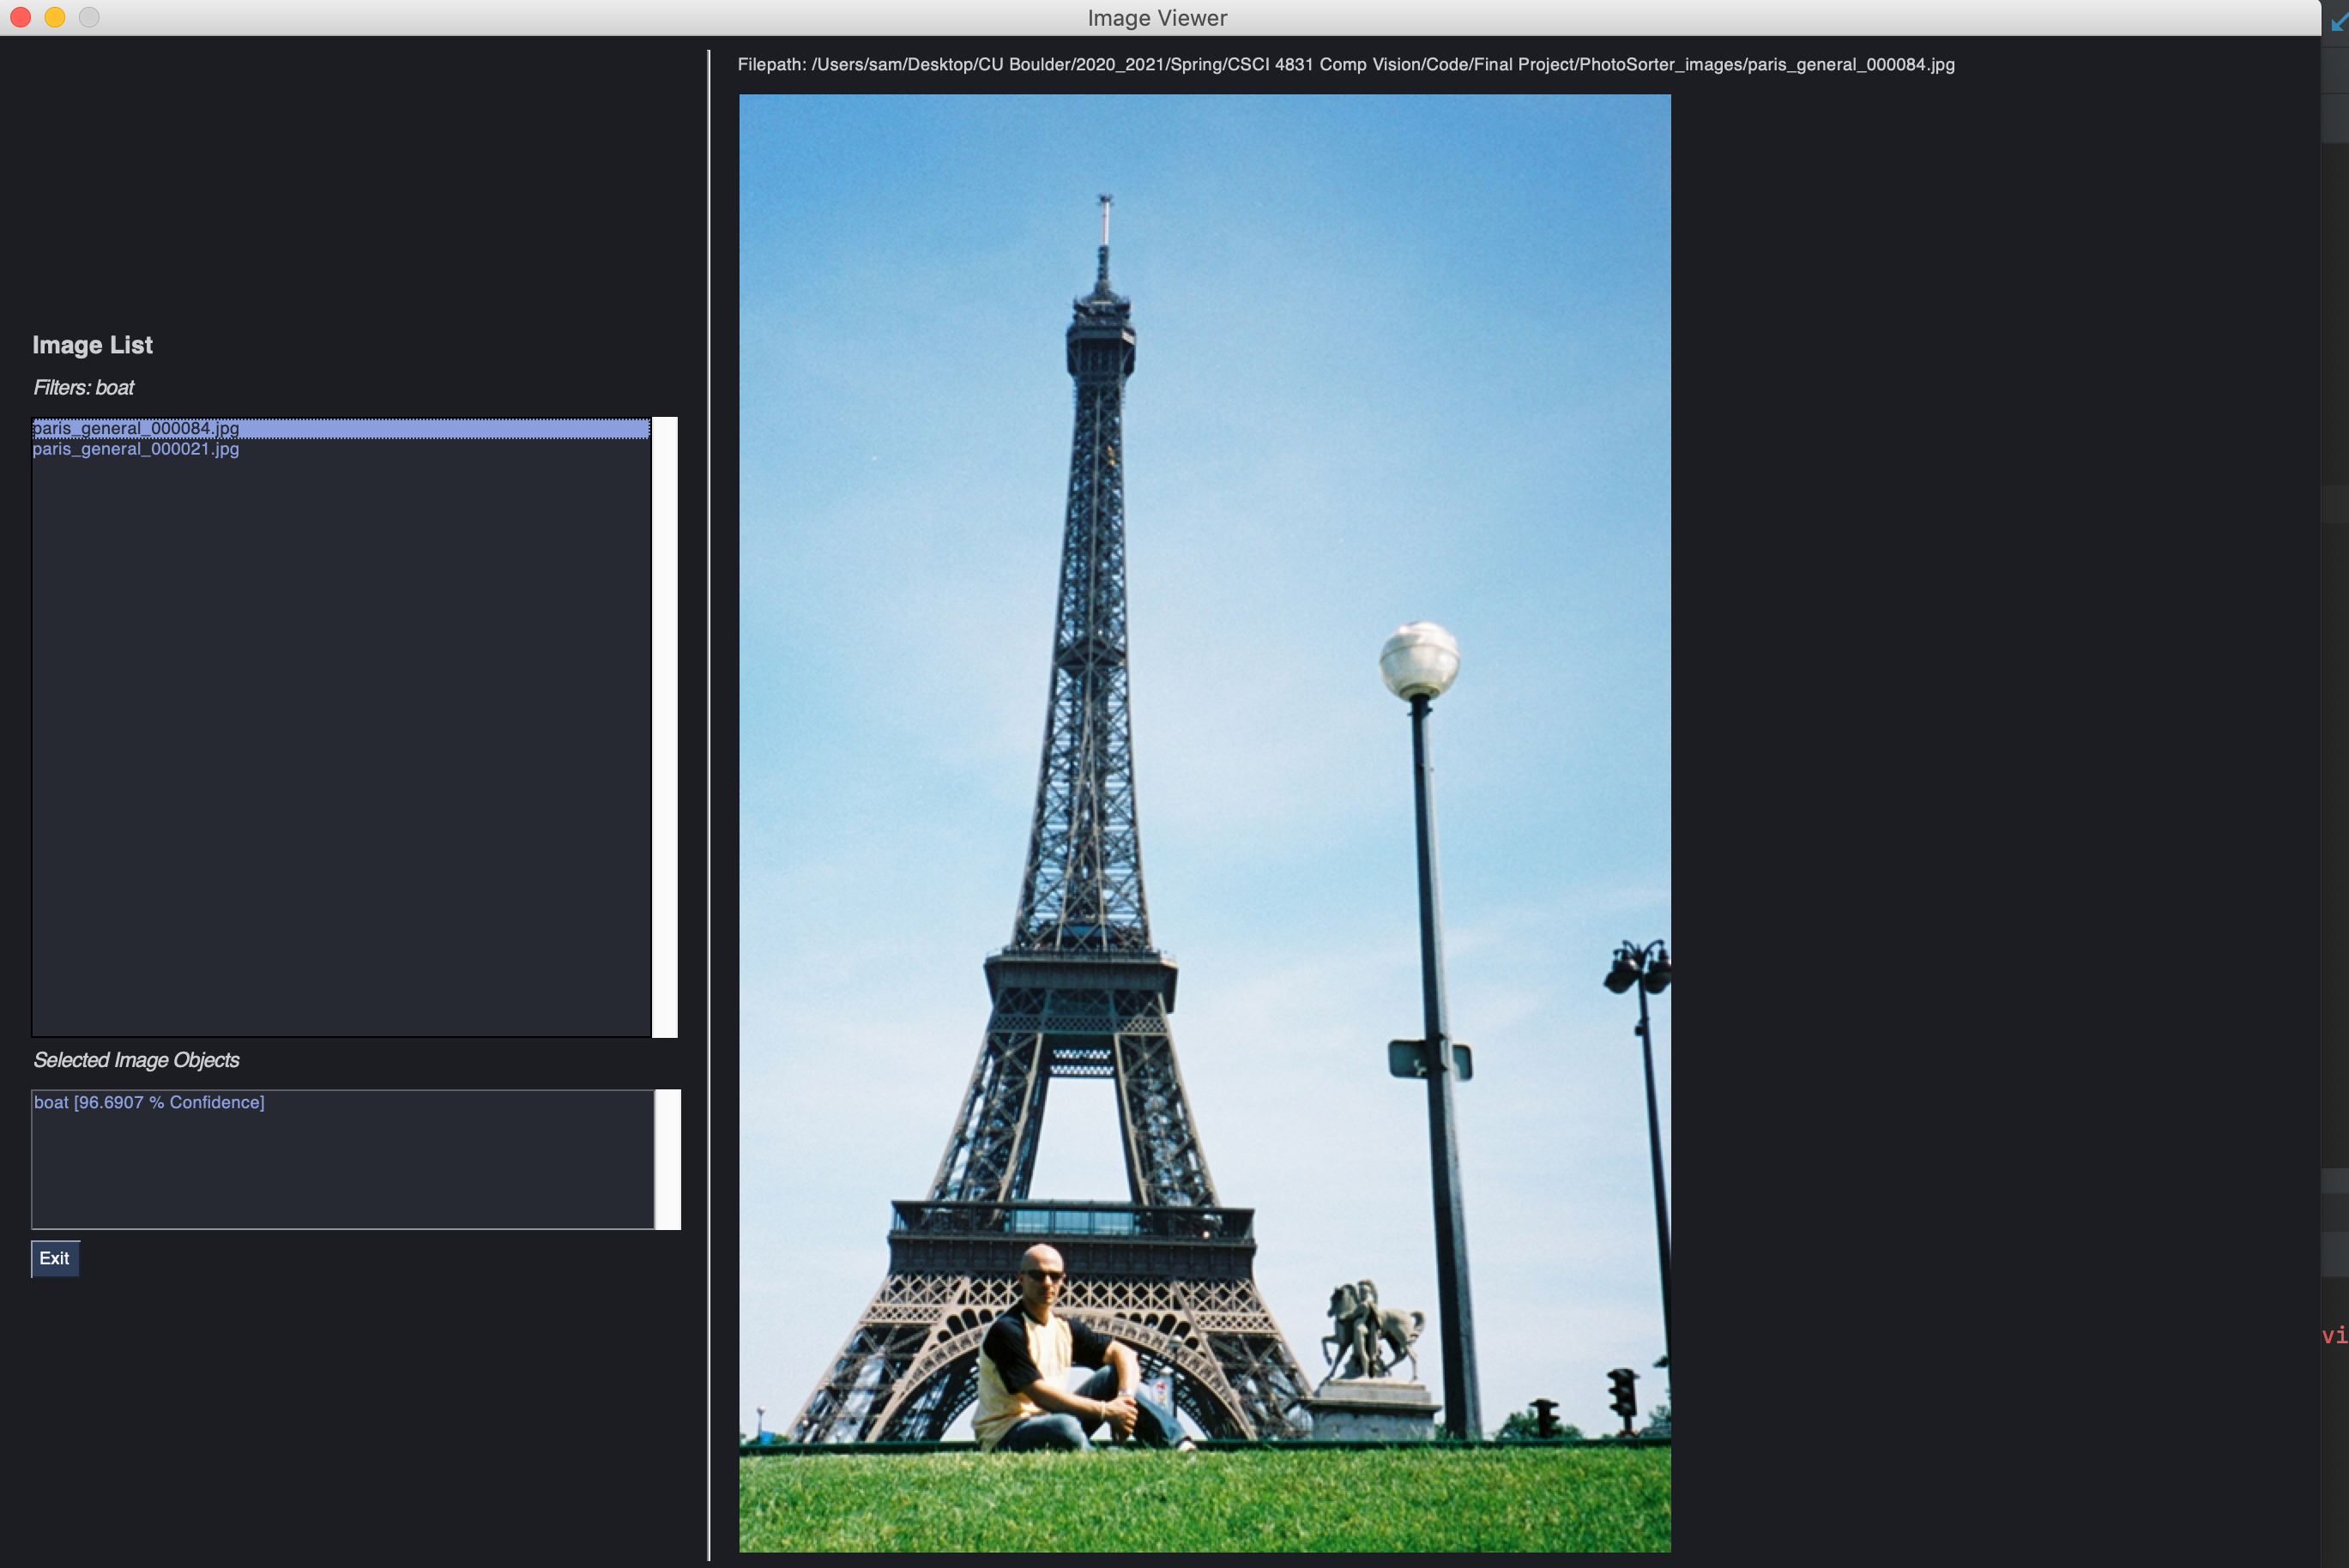
\includegraphics[scale=0.3]{images/incorrect_classification_boat.jpg}


\section{Computer Vision Methods}
\subsection{Near Duplicate Matching}

	We attempted using two different feature detection algorithms in our project. First was Scale-Invariant Feature Transform (SIFT), and the other was Oriented FAST and Rotated BRIEF (ORB). We tried using ORB as it was branded as an "efficient alternative to SIFT or SURF". Both are implemented in the code but only SIFT is actively used due to issues encountered with ORB.
	
	In the end, our near duplicate photo sorting algorithm uses Scale-Invariant Feature Transform (SIFT) to do keypoint and description generation for the features in the image. In OpenCV's SIFT implementation, feature descriptors are a matrix of neighbors to the feature pixel. These can then be matched using a nearest neighbors algorithm to determine feature matches. 
	
	OpenCV has a brute force matcher (BFBatcher), and a Fast Library for Approximate Nearest Neighbors matcher (FLANN). Our program's feature matching uses a FLANN based matcher to compute feature descriptor matches due to the increased speed that FLANN provides on large data sets with high dimensional features. We are using FLANN with the FLANN\_INDEX\_KDTREE algorithm and 5 trees. FLANN runs k nearest neighbors with k=2 on the descriptors for the two images it is passed and returns a list (in this case of the best 2) descriptors that matched for each descriptor from a feature in the first image.
	
	From this list of feature matches, they get narrowed down using a ratio test, eliminating all but the best feature matches with a ratio of 0.7 (ie: our best match must be  sufficiently different from the second match to keep it). This helps to prevent ambiguous matching of features improving accuracy.

\subsection{Object Detection}
	

\subsection{Limitations}
	One major limitation of our implementation of the near duplicate matching is in its run time. Despite using the faster FLANN based matcher for kNN, the algorithm still takes a long time to run for checking each image against another (which has to be done many times). This means that the more images it must check, the longer the program will need to run to do the matching for each image. 
	
	In addition, when attempting to use the apparently more efficient algorithm ORB, we hit issues with it not producing enough feature matches to effectively match images together. It produces feature matches numbering in the 20-150 range, whereas when matching an image using SIFT features, it typically had between 4,000-50,000 feature matches. This meant that accuracy with ORB was a problem and lead to a lot of miss-matching of images when doing the nearest neighbor matching.


\section{Analysis}

\subsection{Individual Contribution}


\subsection{Unsuccessful Attempts}
\subsection{Lessons Learned}

\subsection{Advice for Future Students}

\section*{References}
\end{document}

